\hsection{Programming with Python}%
%
The center of this course is the \python\ programming language.
Our goal is to get familiar with programming, with the programming language \python, and with the tools and ecosystem surrounding it.
This makes sense for several reasons.

\begin{figure}%
\centering%
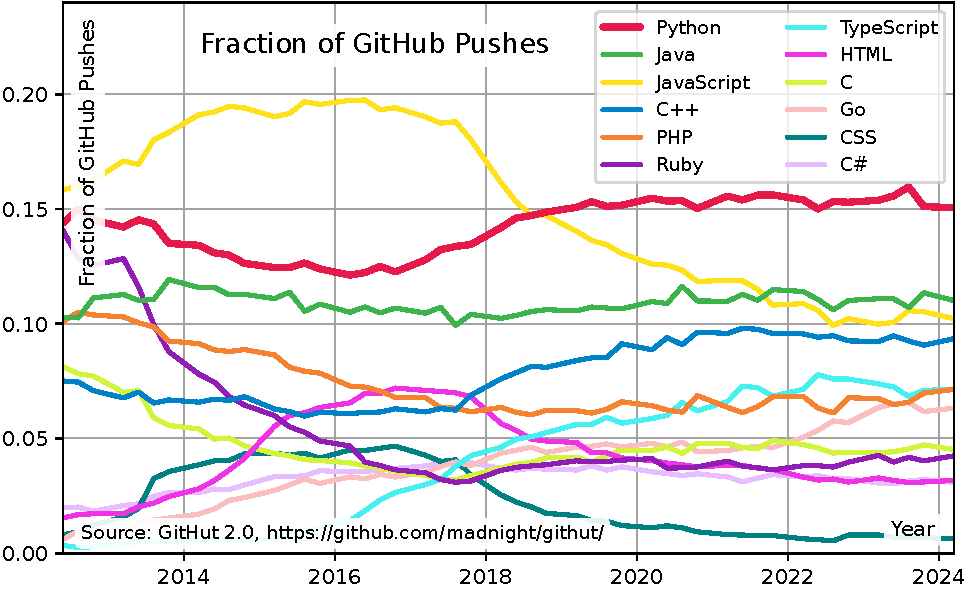
\includegraphics[width=0.75\linewidth]{\currentDir/languagesByGithubPushes}%
\caption{The twelve most popular programming languages chosen based on the \github\ pushes over the years. Source:~\cite{B2023G2GLS}.}%
\label{fig:languagesByGithubPushes}%
\end{figure}%
%
First, \python\ is one of the most successful and widely used programming languages~\cite{CBST2024LOHPPTDDSAMLA}.
If we plot the number of pushes to \github\ over time, we find that \python\ became the leading languages at some point in 2018.
\python\ is intensely used in the fields of \pgls{AI}, \pgls{ML}, and \pgls{DS}~\cite{CBST2024LOHPPTDDSAMLA} as well as optimization, which are among the most important areas of future technology.
There exists a very large set of powerful libraries supporting both research and application development in these fields, including \numpy~\cite{HMvdWGVCWTBSKPHvKBHFdRWPGMSRWAGO2020APWN}, \pandas~\cite{B2012DPWP}, \scikitlearn~\cite{PVGMTGBPWDVPCBPD2011SMLIP}, \scipy~\cite{VGOHRCBPWBvdWBWMMNJKLCPFMVLPCHQHARPvMS2020SFAFSCIP}, \tensorflow~\cite{ABCCDDDGIIKLMMMSTVWWYZ2016TASFLSML}, \matplotlib~\cite{H2007MA2GE}, and \moptipy~\cite{WW2023RSDEWASSAA}.
Learning \python\ can be useful for a wide variety of reasons.
If you will do programming in any future employment or research position, chances are that \python\ knowledge will be useful.%
%
\endhsection%
%
